\section{Observation and Calculations}

\subsection{Gain Variations at a fixed wavelength}
Here, Table I shows the output vs. supplt voltage of the PMT. Using the relation between gain and two voltages, we can rewrite the equation to find the value of $\alpha n$.
\begin{align*}
    \log G = \alpha n \log V + \log K'
\end{align*}

\begin{table}[H]
    \centering
    \begin{tabular}{|c|c|c|c|c|}
    \hline
    $V_{Supply}$ (V) & $V_{O/P}$ (V) & Gain & log G & log V \\ \hline
    0.30 & 0.96 & 3.20 & 0.5051 & -0.5229 \\ 
    0.35 & 2.18 & 6.23 & 0.7944 & -0.4559 \\ 
    0.40 & 7.21 & 18.03 & 1.2559 & -0.3979 \\ 
    0.45 & 11.70 & 26.00 & 1.4150 & -0.3468 \\ 
    0.50 & 17.10 & 34.20 & 1.5340 & -0.3010 \\ 
    0.55 & 31.10 & 56.55 & 1.7524 & -0.2596 \\ 
    0.60 & 41.90 & 69.83 & 1.8441 & -0.2218 \\ 
    0.65 & 55.00 & 84.62 & 1.9274 & -0.1871 \\ 
    0.70 & 69.10 & 98.71 & 1.9944 & -0.1549 \\ \hline

\end{tabular}
\caption{Current gain in output DSO}
\end{table}

\begin{figure}[H]
    \centering
    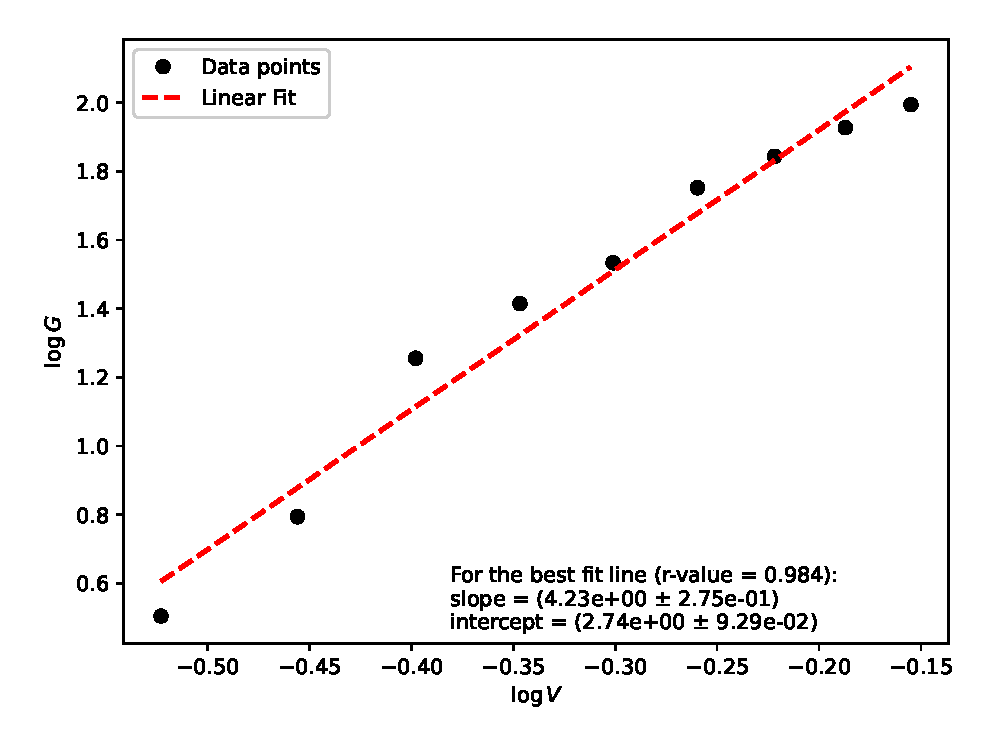
\includegraphics[width=1\columnwidth]{images/gain.eps}
    \caption{Plot for gain Response for 600 nm}
    \label{g1}
\end{figure}

By applying least square fitting, we can approximate a linear fit for $\log G$ vs. $\log V$ (Fig. 3) and estimate the value of $\alpha n = 4.231$.
\vspace{-2em}
\subsection{Spectral Response}

Tables II and III show the wavelength dependednt characteristics of the LED and the PMT. Using these, the sensitivity of the PMT at different wavelengths were calculated and plotted (Fig. 4). We can see that the highest sensitivity is for blue light (460 nm) and there is a significant dip for yellow light (570 nm) after which it increases.
Also note the high measurement uncertainty in the sensitivity values, which are primarily because of the high variation in the observed parameters and the high least counts of the instruments.

\begin{table}[H]
    \centering
    \begin{tabular}{|c|c|c|c|c|c|}
    \hline
    $\lambda$ (nm) & $V_{LED}$ (V) & $I_{LED}$ (mA) & $ P_{LED}$ (W) & $V_{PD}$ (V) & $I_{PD}$ (mA)  \\ \hline
    460 & 1.090 & 138.4 & 0.151 & 192.3 & 0.1 \\
    500 & 0.889 & 125.6 & 0.112 & 186.9 & 0.1 \\
    540 & 0.696 & 115.1 & 0.080 & 179.5 & 0.1 \\
    570 & 0.669 & 113.3 & 0.076 & 176.1 & 0.1 \\
    635 & 0.598 & 115.2 & 0.069 & 184.4 & 0.1 \\ \hline

    \end{tabular}
\caption{Wavelength-dependent characteristics of LED and Photodetector}
\end{table}
\begin{table}[H]
    \centering
    \begin{tabular}{|c|c|c|c|c|c|}
    \hline
    $\lambda$ (nm) & $V_{PMT}$ (mV) & $I_{PMT}$ (A) & $ S_{PMT}$ (A/W) \\ \hline
    460 & 800 & 0.800 & 5.303 \\
    500 & 520 & 0.520 & 4.657 \\
    540 & 280 & 0.280 & 3.495 \\
    570 & 180 & 0.180 & 2.375 \\
    635 & 320 & 0.320 & 4.645 \\ \hline

    \end{tabular}
\caption{Wavelength-dependent characteristics of PMT}
\end{table}

\begin{figure}[H]
    \centering
    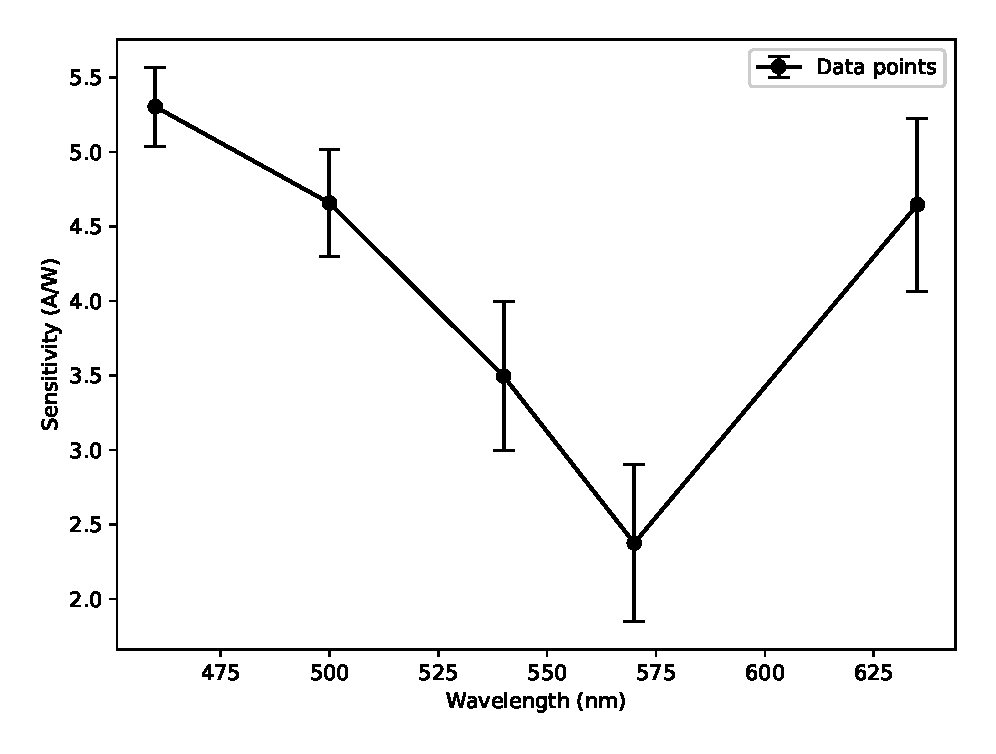
\includegraphics[width=1\columnwidth]{images/spec.eps}
    \caption{Plot for anode sensitivity vs. wavelength}
    \label{g2}
\end{figure}

\subsection{Dark Current}
The anode dark current was measured at various
control voltages while ensuring that the PMT was
completely isolated from external light sources (Table IV and Fig. 5).

\begin{table}[H]
    \centering
    \begin{tabular}{|c|c|}
    \hline
    $V_{PMT}$ (mV) & $I_{PMT}$ (A) \\ \hline
    0.5 & 0.0 \\
    0.6 & 0.2 \\
    0.7 & 0.8 \\
    0.8 & 1.4 \\
    0.9 & 6.2 \\
    1.0 & 14.1 \\ \hline
\end{tabular}
\caption{Dark current vs supply voltage in PMT}
\end{table}
\begin{figure}
    \centering
    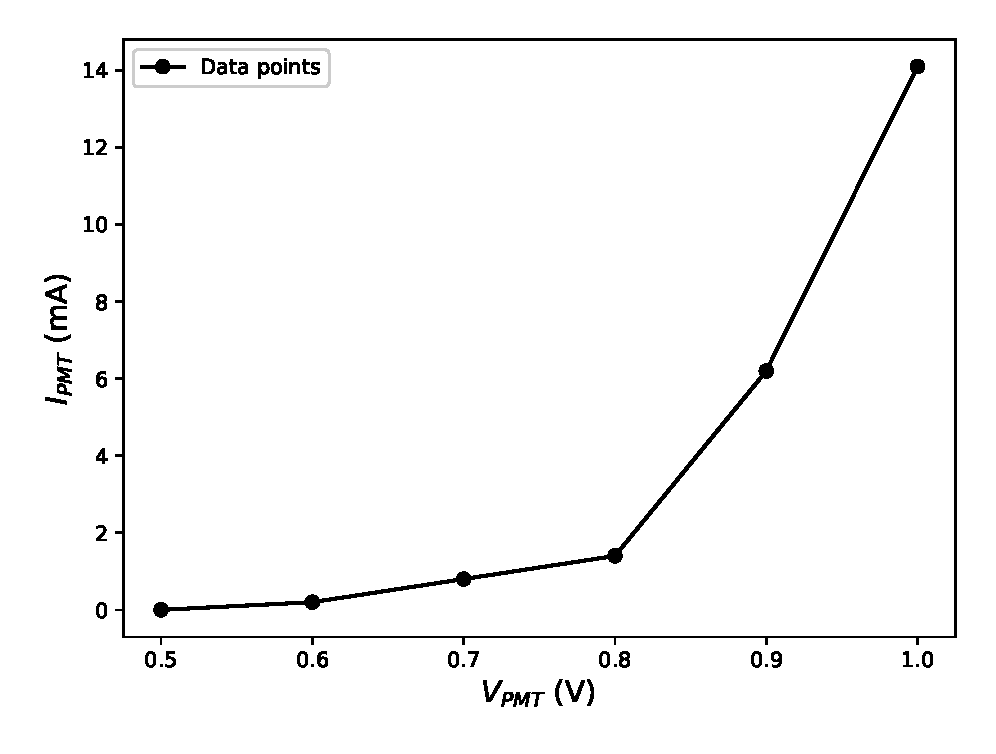
\includegraphics[width=1\columnwidth]{images/dark.eps}
    \caption{Dark current vs supply voltage in PMT}
    \label{g3}
\end{figure}

\section{Error Analysis}
Since $\alpha n$ is obtained from a linear fit, its uncertainty
$\Delta (\alpha n)$ can be determined from the standard error propagation formula for the slope in linear regression.

\begin{align*}
    \frac{\Delta (\alpha n)}{ (\alpha n)} = \frac{\Delta \text{slope}}{\text{slope}}
\end{align*}

which comes out to be the same as $\Delta \text{slope} = \Delta (\alpha n) = 0.275$.